\chapter{Single top quark production with a photon in the Standard Model}
\section{A brief overview of the standard model}
\section{The \texorpdfstring{$tq\gamma$}{TEXT} process in the standard model}


\chapter{Measurement of \texorpdfstring{$tq\gamma$}{TEXT}}



\section{The ATLAS Experiment}

The European Organization for Nuclear Research, known as CERN, located in Geneva, has various experiments studying elementary particles through the collision of heavy ions and protons. 
The Large Hadron Collider (LHC), the particle accelerator of CERN, has a circumference of $27 \si{\kilo\metre}$ and can collide particles with an energy of up to $13.6 \si{\tera\electronvolt}$. 


The LHC consists of four extensive experiments: the ALICE, the LHCb, the CMS and the ATLAS experiments. The research in this paper is done with the help of the largest of these experiments, the ATLAS experiment. Figure 1 visualizes the structure of the ATLAS detector.  The detector is built symmetrically around the particle beam divided into three subdetectors.

The inner detector tracks charged particles just after the collision. It consists of three different systems of sensors in a magnetic field parallel to the beam. These sensors are the pixel detector, the semiconductor tracker that works with silicon strips and a transition radiation tracker to track particles with gas-filled tubes. 

The calorimeters detect showers produced by electrons, photons and hadrons. 

The muon spectrometer measure trajectories of muons with the help of a magnetic field. The spectrometer detects muons in the range of $\bigl|\nu\bigr| = 2.7$. 
Monitured drift tubes are used up to $\nu = 2.0$ and cathode strip chambers are used for higher pseudorapidities.  
\begin{figure}
    \centering
    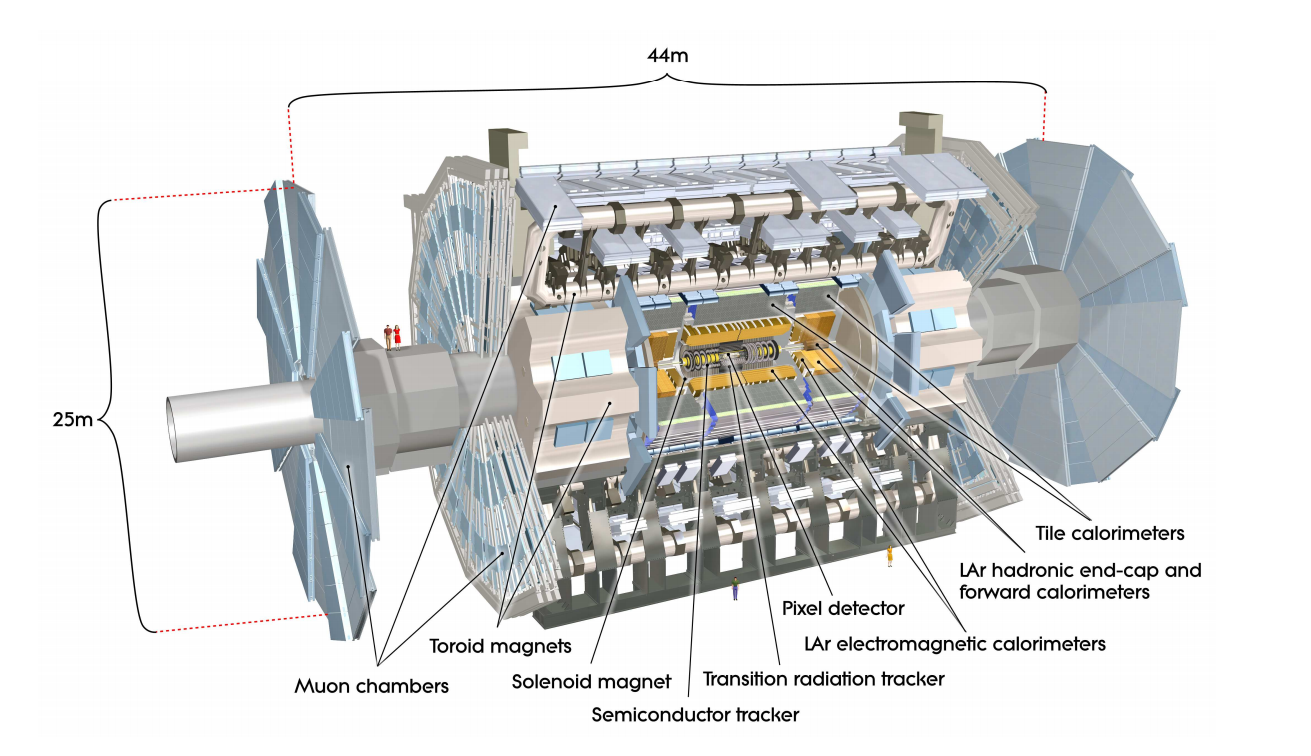
\includegraphics[width=0.9\textwidth]{Plots/atlasSCHEMA.PNG}
    \label{fig:atlasschema}
    \caption{Schematic visualisation of the ATLAS Detector \cite{Collaboration_2008}.}
\end{figure}



\section{Object Reconstruction at the ATLAS experiment}
\section{Background contributions from similar processes}





\chapter{Monte Carlo samples and event selection}
\section{Generation of Monte Carlo samples}
\section{Event selection}
\chapter{The Neural Network used for signal-background classification}
\section{How a neural network works}
\section{The NN architecture}
\section{Input features for the neural network}
\section{NN Efficiancy and distribution of the NN output}
\chapter{Analysis of the effects of different event feautures on the neural network output}
\section{Correlations of input feautures with the NN output}
\section{Changes in the NN output distribution for different photon \texorpdfstring{$p_T$}{TEXT} and fjet+photon energy bins}
\section{?}
\chapter{Conclusions}